\documentclass[]{article}
\hyphenation{co-rres-pon-dien-tes te-ner E-ben-sper-ger de-pre-da-do-res dis-po-ni-ble be-ne-fi-cio-sa in-di-vi-dual so-cia-li-dad mos-tra-ron fuen-tes a-cep-ta-ble ta-ma-ño o-pues-ta mo-de-lo es-tu-dian-tes e-jer-ci-cios co-rres-pon-dien-te mo-di-fi-ca-dos mo-di-fi-car-lo ma-ni-pu-lar}
\usepackage[T1]{fontenc}
\usepackage{lmodern}
\usepackage{amssymb,amsmath}
\usepackage{ifxetex,ifluatex}
\usepackage{fixltx2e} % provides \textsubscript
% use microtype if available
\IfFileExists{microtype.sty}{\usepackage{microtype}}{}
\ifnum 0\ifxetex 1\fi\ifluatex 1\fi=0 % if pdftex
  \usepackage[utf8]{inputenc}
\else % if luatex or xelatex
  \usepackage{fontspec}
  \ifxetex
    \usepackage{xltxtra,xunicode}
  \fi
  \defaultfontfeatures{Mapping=tex-text,Scale=MatchLowercase}
  \newcommand{\euro}{€}
\fi
\usepackage{color}
\usepackage{fancyvrb}
\DefineShortVerb[commandchars=\\\{\}]{\|}
\DefineVerbatimEnvironment{Highlighting}{Verbatim}{commandchars=\\\{\}}
% Add ',fontsize=\small' for more characters per line
\newenvironment{Shaded}{}{}
\newcommand{\KeywordTok}[1]{\textcolor[rgb]{0.00,0.44,0.13}{\textbf{{#1}}}}
\newcommand{\DataTypeTok}[1]{\textcolor[rgb]{0.56,0.13,0.00}{{#1}}}
\newcommand{\DecValTok}[1]{\textcolor[rgb]{0.25,0.63,0.44}{{#1}}}
\newcommand{\BaseNTok}[1]{\textcolor[rgb]{0.25,0.63,0.44}{{#1}}}
\newcommand{\FloatTok}[1]{\textcolor[rgb]{0.25,0.63,0.44}{{#1}}}
\newcommand{\CharTok}[1]{\textcolor[rgb]{0.25,0.44,0.63}{{#1}}}
\newcommand{\StringTok}[1]{\textcolor[rgb]{0.25,0.44,0.63}{{#1}}}
\newcommand{\CommentTok}[1]{\textcolor[rgb]{0.38,0.63,0.69}{\textit{{#1}}}}
\newcommand{\OtherTok}[1]{\textcolor[rgb]{0.00,0.44,0.13}{{#1}}}
\newcommand{\AlertTok}[1]{\textcolor[rgb]{1.00,0.00,0.00}{\textbf{{#1}}}}
\newcommand{\FunctionTok}[1]{\textcolor[rgb]{0.02,0.16,0.49}{{#1}}}
\newcommand{\RegionMarkerTok}[1]{{#1}}
\newcommand{\ErrorTok}[1]{\textcolor[rgb]{1.00,0.00,0.00}{\textbf{{#1}}}}
\newcommand{\NormalTok}[1]{{#1}}
\usepackage{graphicx}
% We will generate all images so they have a width \maxwidth. This means
% that they will get their normal width if they fit onto the page, but
% are scaled down if they would overflow the margins.
\makeatletter
\def\maxwidth{\ifdim\Gin@nat@width>\linewidth\linewidth
\else\Gin@nat@width\fi}
\makeatother
\let\Oldincludegraphics\includegraphics
\renewcommand{\includegraphics}[1]{\Oldincludegraphics[width=\maxwidth]{#1}}
\ifxetex
  \usepackage[setpagesize=false, % page size defined by xetex
              unicode=false, % unicode breaks when used with xetex
              xetex]{hyperref}
\else
  \usepackage[unicode=true]{hyperref}
\fi
\hypersetup{breaklinks=true,
            bookmarks=true,
            pdfauthor={},
            pdftitle={},
            colorlinks=true,
            urlcolor=blue,
            linkcolor=magenta,
            pdfborder={0 0 0}}
\setlength{\parindent}{0pt}
\setlength{\parskip}{6pt plus 2pt minus 1pt}
\setlength{\emergencystretch}{3em}  % prevent overfull lines
\setcounter{secnumdepth}{0}

\author{}
\date{}

\begin{document}

\section{Ejercicios de programación IV: Gráficos y estadística}

\subsubsection{{[}IMSER 2013{]}}

\begin{center}\rule{3in}{0.4pt}\end{center}

\subsection{Archivos incluidos:}

El archivo con los ejercicios del práctico debe bajarse y descomprimirse
en disco duro, creando la carpeta \textbf{\texttt{rep-X}} (nota: no debe
dentro de ningún disco, partición o carpeta protegida a la escritura,
como puede ser un disco duro externo de backup). Usted deberá abrir el
RStudio y seleccionar dicha carpeta como su directorio de trabajo con
\texttt{setwd} o en RStudio la combinación \textbf{Ctrl + Shift + K}. En
esta carpeta se encuentran algunos archivos que usted deberá modificar:

\begin{itemize}
\item
  \textbf{\texttt{1.a-genero.R}}
\item
  \textbf{\texttt{1.b-hist.R}}
\item
  \textbf{\texttt{1.c-cajas.R}}
\item
  \textbf{\texttt{1.d-regresion.R}}
\item
  \textbf{\texttt{1.e-dispersion.R}}
\end{itemize}

Adicionalmente los siguientes archivos son necesarios, pero \textbf{no
deben ser modificados} para que el método de calificación automático
funcione correctamente.

\begin{itemize}
\item
  \texttt{evaluar.R}
\item
  \texttt{datos}
\item
  \texttt{INSTRUCCIONES.pdf}
\item
  \texttt{hacemagia.R}
\item
  \texttt{auxiliar.RData}
\end{itemize}

\subsection{Mecanismo de corrección:}

Nota: más recomendaciones \textbf{importantes} se hacen en el documento
\href{http://goo.gl/P5Wnq}{Dinámica de los repartidos}.

Lo primero que debe hacer es cargar el archivo evaluar.R con la función
\texttt{source} y la codificación de caracteres ``UTF-8'' (lo cual
afecta a la función \texttt{evaluar} en particular), de la siguiente
manera:

\begin{Shaded}
\begin{Highlighting}[]
\KeywordTok{source}\NormalTok{(}\StringTok{"evaluar.R"}\NormalTok{, }\DataTypeTok{encoding =} \StringTok{"UTF-8"}\NormalTok{)}
\end{Highlighting}
\end{Shaded}

Nótese que hemos dejado de usar la función \texttt{options}, de forma
que de ahora en más \textbf{no ejecute el comando}:

\begin{Shaded}
\begin{Highlighting}[]
\KeywordTok{options}\NormalTok{(}\DataTypeTok{encoding =} \StringTok{"utf-8"}\NormalTok{)  }\CommentTok{# No me ejecuten!}
\end{Highlighting}
\end{Shaded}

Este cambio se debe a que hemos detectado que esta elección trae más
problemas que soluciones.

Si usted ha ejecutado todos los pasos anteriores correctamente, al usar
el comando \texttt{ls()} verá que \texttt{"evaluar"} figura en su sesión
y además en la consola debería ver lo siguiente:

\begin{verbatim}
Archivo de código fuente cargado correctamente

Chequeo de encoding:
  Los siguientes caracteres deben ser vocales con tilde:
    á - é - í - ó - ú
  Si *no se ven correctamente* corra el siguiente comando:
    source('evaluar.R', encoding = 'UTF-8')
\end{verbatim}

Usted trabajará modificando los contenidos de los archivos de los
ejercicios con RStudio (u otro programa de su preferencia) según las
consignas que se describen a continuación. Luego de terminar cada
ejercicio y \textbf{guardando el archivo} correspondiente en el disco
duro, usted podrá verificar rápidamente si su respuesta es correcta
ejecutando el comando:

\begin{Shaded}
\begin{Highlighting}[]
\KeywordTok{evaluar}\NormalTok{()}
\end{Highlighting}
\end{Shaded}

y además podrá en todo momento verificar su puntaje con la función
\texttt{verNotas()}. Tenga siempre en cuenta que, a \textbf{menos que
sea indicado} por la letra del ejercicio, las soluciones deben ser
genéricas y por lo tanto deben servir aún si se modifican los datos
originales (i.e.: no use valores fijos si no comandos). Usualmente se
utilizan valores generados de forma aleatoria para las correcciones
automáticas. Los objetos que son evaluados en la corrección automática
estarán indicados con un asterísco en las instrucciones de cada script.
Nótese además que en los archivos \textbf{se indica claramente en dónde
se inicia y dónde finaliza su código} y que debe respetar esta
organización para que la corrección de los ejercicios funcione bien.

\subsubsection{Al finalizar}

Una vez terminados y guardados los archivos de los ejercicios del
repartido, usted deberá ejecutar \texttt{evaluar()} y seleccionar la
última opción (``Todos'') y luego subir el archivo ''datos'' (sin
extensión), incluido en la carpeta ''rep-1'', a la
\href{http://eva.universidad.edu.uy/mod/assign/view.php?id=103966}{sección
de entregas} de la portada del curso en la plataforma EVA. Este archivo
se podrá reemplazar con uno más nuevo, en caso de que desee corregir
algún error; en caso de querer que el archivo sea corregido antes de la
fecha de entrega, puede cambiarle el nombre a ``datos-finalizado'', pero
en ese caso la nota no se cambiará de ahí en adelante.

\subsubsection{Código de Honor}

Si bien animamos a que trabaje en equipos y que haya un intercambio
fluido en los foros del curso, es fundamental que las respuestas a los
cuestionarios y ejercicios de programación sean fruto del trabajo
individual. En particular, consideramos necesario que no utilice el
código creado por sus compañeros, si no que debe programar sus propias
instrucciones, ya que de lo contrario supone un sabotaje a su propio
proceso de aprendizaje. Esto implica también evitar, en la medida de lo
posible, exponer el código propio a sus colegas. Como profesores estamos
comprometidos a dar nuestro mayor esfuerzo para dar las herramientas y
explicaciones adecuadas a fin de que pueda encontrar su propio camino
para resolver los ejercicios.

En casos de planteos de dudas a través del foro, en los que considere
que es imposible expresar un problema sin exponer su própio código,
entonces es aceptable hacerlo. De todas formas en estos casos es
preferible que envíe su código por correo electrónico directamente a un
profesor, explicando la problemática.

\begin{center}\rule{3in}{0.4pt}\end{center}

\subsection{1. Campeonato de Magic}

El juego
\href{https://es.wikipedia.org/wiki/Magic:\_el\_encuentro}{Magic: el
encuentro}, popular entre muchos jóvenes aficionados a los generos
literarios de fantasía y los juegos de rol, congrega campeonatos
mundiales regularmente. Pensando en estos campeonatos, creamos una
data.frame de datos ficticios de los participantes. Para a agregar a su
sesión de R una data.frame llamada \texttt{magic} con dichos datos,
ejecute:

\begin{Shaded}
\begin{Highlighting}[]
\KeywordTok{source}\NormalTok{(}\StringTok{"hacemagia.R"}\NormalTok{)}
\end{Highlighting}
\end{Shaded}

A partir de esta data.frame haremos varios análisis sencillos y algunos
gráficos correspondientes.

\subsubsection{1.a Variable ``genero''}

La variable \texttt{genero} de la data.frame presenta los valores 1 y 2.
Transforme esta variable en factor y luego modifique los nombres de los
niveles del mismo a \texttt{"mujer"} y \texttt{"hombre"}
(correspondientes a los valores originales 1 y 2 respectivamente).

Por ejemplo, la variable original:

\begin{Shaded}
\begin{Highlighting}[]
\NormalTok{>}\StringTok{ }\NormalTok{magic$genero[}\DecValTok{1}\NormalTok{:}\DecValTok{4}\NormalTok{]}
\NormalTok{[}\DecValTok{1}\NormalTok{] }\DecValTok{1} \DecValTok{2} \DecValTok{1} \DecValTok{2}
\end{Highlighting}
\end{Shaded}

\ldots{} y la variable modificada:

\begin{Shaded}
\begin{Highlighting}[]
\NormalTok{>}\StringTok{ }\NormalTok{magic$genero[}\DecValTok{1}\NormalTok{:}\DecValTok{4}\NormalTok{]}
\NormalTok{[}\DecValTok{1}\NormalTok{] mujer  hombre mujer  hombre}
\NormalTok{Levels:}\StringTok{ }\NormalTok{mujer hombre}
\end{Highlighting}
\end{Shaded}

\subsubsection{1.b Histogramas}

Nota: la corrección de este ejercicio asume que usted ya cambió la
columna \texttt{genero} según las instrucciones de 1.a.

Aquí debe hacer un gráfico como el de la figura 1. Se trata de dos
histogramas de los valores de alturas de los participantes, separados
por sexo. En el histograma de arriba se encuentran las alturas de las
mujeres, y de los hombres en el de abajo. Para lograr este gráfico hay
que comprender al menos dos comandos:

\paragraph{i. función \texttt{par}}

Con la función \texttt{par} se pueden determinar la cantidad de gráficos
que vamos a tener dentro de cada figura. Para eso se usa alguno de los
parámetros \texttt{mfcol} o \texttt{mfrow} (no al mismo tiempo). Utilice
estos parámetros correctamente para lograr dividir la figura en dos
gráficos tal como en el ejemplo.

\begin{figure}[htbp]
\centering

\includegraphics{figure/unnamed-chunk-8.png}
\caption{Histograma de las alturas de mujeres y hombres (ej. 1.b)}
\end{figure}

\paragraph{ii. función \texttt{hist}}

Con la función \texttt{hist} usted puede graficar rápidamente un
histograma en R. En este caso tiene que utilizar los valores de altura,
pero recuerde \textbf{separar por hombres y mujeres} antes de hacer los
dos histogramas. Por otro lado debe fijar la cantidad de celdas/cortes
en \emph{25}, utilizando el argumento correcto de la función. Es posible
que en la figura final este número no coincida con la cantidad de
barras, ya que actúa tan sólo como una sugerencia para \texttt{hist}.

Nota: la cantidad de cortes asignada parece una exageración, pero se
trata de un número que sirve a los propósitos de la corrección
automática.

\subsubsection{1.c Gráfico de cajas}

En este ejercicio simplemente vamos a graficar utilizando los argumentos
que editan los títulos de los gráficos. La idea es hacer un gráfico de
cajas del peso de los participantes en función de su género, poniendo
textos adecuados para el mismo. Estos textos serán los siguientes:

\begin{itemize}
\item
  Título: ``Peso en funcion del genero''
\item
  Etiqueta del eje horizontal: ``Genero''
\item
  Etiqueta del eje vertical: ``Peso (Kg)''
\end{itemize}

(Se omiten las comas para evitar problemas de encoding.)

Recuerde que para agregar estos elementos debe utilizar los parámetros
gráficos de R, los cuales aparecen listados en la ayuda de la función
\texttt{par}. Estos parámetros se utilizan como argumentos al momento de
llamar a plot, por ejemplo:

\begin{Shaded}
\begin{Highlighting}[]
\KeywordTok{plot}\NormalTok{(speed ~}\StringTok{ }\NormalTok{dist, }\DataTypeTok{data =} \NormalTok{cars, }\DataTypeTok{col =} \StringTok{"red"}\NormalTok{)}
\end{Highlighting}
\end{Shaded}

Aquí se utiliza el parámetro \texttt{col} como argumento de
\texttt{plot}, asignándole el valor ``red''. Nótese que también se
pueden asignar parámetros con comandos del tipo
\texttt{par(parametro = "valor")}, pero en este ejercicio no está
contemplada esta opción, por lo que no debe utilizarla.

Para hacer este gráfico tanto \texttt{plot} como \texttt{boxplot} son
opciones válidas. Recuerde respetar mayúsculas y minúsculas en los
textos, así como la ausencia de tildes. La corrección sólo contempla el
uso de objetos de clase ``formula'' para hacer el plot. Es decir, debe
nombrar las variables siguiendo el esquema
\texttt{y \textasciitilde{} x}, como en el ejemplo anterior (use
\texttt{?plot.formula} para ver la documentación). También es necesario
que utilice el nombre del argumento \texttt{data} para indicar el
data.frame (i.e.: \texttt{data = magic}).

Por último, las variables deben ser los nombres de las columnas: no
sirven opciones como \texttt{cars\$dist} o \texttt{cars{[},2{]}}; debe
usarse directamente \texttt{dist}.

\begin{figure}[htbp]
\centering
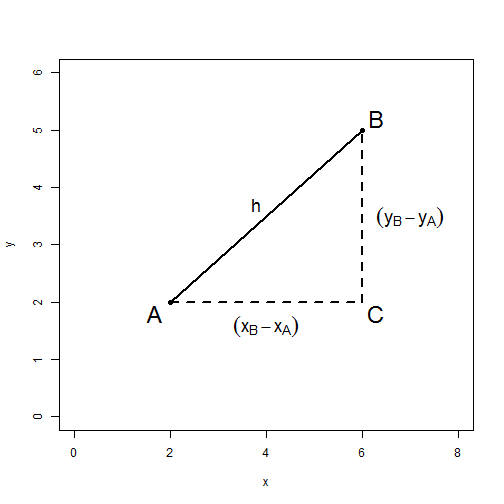
\includegraphics{figure/unnamed-chunk-10.png}
\caption{Gráfico de cajas (ej. 1.c)}
\end{figure}

Nota: si no tiene hecha la parte 1.a puede cargar una data.frame
\texttt{magic} auxiliar con el comando:

\begin{Shaded}
\begin{Highlighting}[]
\KeywordTok{load}\NormalTok{(}\StringTok{"auxiliar.RData"}\NormalTok{)}
\end{Highlighting}
\end{Shaded}

\subsubsection{1.d Regresiones lineales}

En este ejercicio usted hará la regresión lineal entre dos variables: la
altura elevada al cuadrado (\emph{variable de respuesta}) en función del
peso (\emph{variable explicativa}) de los participantes del campeonato.
Debido a que lo esperable es que a medida que el peso se aproxima a 0 la
altura también lo haga, la regresión se hará \textbf{sin intercepto}. El
objeto \texttt{reg.a} será esta regresión, la cual debe crearse con la
función \texttt{lm}.

Posteriormente hará otra regresión, pero eliminando outliers
(\texttt{reg.b}; ver fig. 3). Se detectó que hay algunos participantes
con un peso mucho mayor al esperable por su altura. Por eso es más
razonable eliminar estos valores para obtener una regresión que sirva
para hacer predicciones útiles. Haga una regresión idéntica a la
anterior, pero de tal forma que \textbf{no se usen} las filas de
\texttt{magic} tales que el peso es igual o mayor a 95 Kg.

\begin{figure}[htbp]
\centering
\includegraphics{figure/unnamed-chunk-12.png}
\caption{se muestran en rojo los outliers; la recta es reg.b.}
\end{figure}

Con esta segunda regresión ahora usted va a hacer predicciones de
alturas en base un vector de pesos generado aleatoriamente (\texttt{p}).
Considere que si $a$ es la altura y $c$ es el coeficiente obtenido en la
regresión lineal (i.e.: la pendiente de la recta), entonces se debe
cumplir que:

\[
  a ^ 2 = c \cdot p
\]

\[
  a = \sqrt{c \cdot p}
\]

El objeto \texttt{ae} deberá ser un vector con las alturas esperadas
dado el vector de pesos \texttt{p}.

Finalmente guardará el valor del
\href{https://en.wikipedia.org/wiki/Coefficient\_of\_determination}{coeficiente
de determinación} o $R^2$ en el objeto \texttt{r2}. Para obtener este
valor recuerde que la función \texttt{summary} aplicada a objetos
\texttt{lm}\href{i.e.\%20`summary.lm`,\%20aunque\%20por\%20supuesto\%20no\%20hay\%20que\%20poner\%20el\%20`.lm`\%20final,\%20ya\%20que\%20`summary`\%20es\%20una\%20función\%20genérica.}{1}
devuelve un objeto de tipo lista, el cual incluye el valor del $R^2$.
Para ubicar fácilmente en dónde se encuentra este valor en la lista
\texttt{str} puede ser una función muy útil. Por supuesto que también
puede basarse en un libro de texto para hallar este valor.

\subsubsection{1.e Gráfico de dispersión}

En este ejercicio se propone reproducir una figura como la 4. Para eso
el código ya está a medio hacer, usted sólamente necesita ajustar los
objetos que se crean antes de los plots para que se asemeje a lo que se
ve en el ejemplo. Tiene libertad para elegir ciertos parámetros, como
los colores o el tipo de puntos.

De todas formas, el órden en que se pusieron las funciones no es el
correcto, por lo que deberá mover de lugar las líneas de código que se
encuentran bajo el marcador \texttt{\#\#!}. La clave está en identificar
cuáles son funciones de ``alto nivel'' (``High Level Plot functions'') y
cuáles no. Una vez que ordena por alto/bajo nivel, el resto puede
ordenarlo como prefiera.

También podrá agregar nuevos argumentos a los plots, como

\begin{figure}[htbp]
\centering

\includegraphics{figure/unnamed-chunk-13.png}
\caption{Gráfico de dispersión, ej. 1.e}
\end{figure}

Nota: si no tiene hechas las partes 1.a y/o 1.d puede cargar una
data.frame \texttt{magic} auxiliar, así como la regresión \texttt{reg.b}
necesaria, con el comando:

\begin{Shaded}
\begin{Highlighting}[]
\KeywordTok{load}\NormalTok{(}\StringTok{"auxiliar.RData"}\NormalTok{)}
\end{Highlighting}
\end{Shaded}

\subsubsection{1.f Leyenda (sin calificación)}

(\emph{Este ejercicio no se podrá evaluar con el mecanismo de corrección
automática y por lo tanto no entrará en la nota total. Puede
considerarlo simplemente como un ejercicio ``desafío''.})

El objetivo es sencillo: tratar de lograr un resultado similar a la
figura 5. Como este no tiene puntaje es totalmente opcional. Invitamos a
todos los interesados a que usen el foro y compartan sus códigos a fin
de encontrar una solución o posibles mejoras al gráfico en cuestión.

Pistas: para generar el gráfico de ejemplo (fig. 5) se usaron las
siguientes funciones: \texttt{plot}, \texttt{points}, \texttt{abline},
\texttt{legend}, \texttt{text}, \texttt{rug}, \texttt{format},
\texttt{bquote}, \texttt{expression}, \texttt{summary}, \texttt{round},
\texttt{paste0} y algunas otras muy comunes.

\begin{figure}[htbp]
\centering

\includegraphics{figure/unnamed-chunk-15.png}
\caption{el gráfico `desafío', ej. 1.f}
\end{figure}

\end{document}
